\documentclass[conference]{IEEEtran}
\IEEEoverridecommandlockouts
\usepackage{amsmath,amssymb}
\usepackage{graphicx}
\usepackage{cite}
\usepackage{xcolor}
\usepackage{booktabs}
\usepackage{textcomp}

\def\BibTeX{{\rm B\kern-.05em{\sc i}\kern-.025em b\kern-.08em T\kern-.1667em\lower.7ex\hbox{E}\kern-.125emX}}

\begin{document}

\title{GLIMPSE: One-Sided Learned CSI Feedback via a Published Karhunen--Lo\`{e}ve Sketch}

\author{
\IEEEauthorblockN{Author Name\IEEEauthorrefmark{1}}
\IEEEauthorblockA{\IEEEauthorrefmark{1}Department of Electrical and Computer Engineering, University Name, City, Country\\
Email: author@university.edu}
}

\maketitle

\begin{abstract}
The 3GPP Type II CSI codebooks and the two-sided learned-CSI literature both fall short of deployment: codebooks waste bits re-encoding support on a fixed DFT grid, while autoencoders (the CsiNet family) need a UE-side neural network and inter-vendor training/version-matching that 3GPP has not solved. We propose GLIMPSE, a one-sided scheme in which the UE runs zero learned parameters: it reports a fixed, published linear sketch -- the top-$m$ rows of the channel's Karhunen--Lo\`{e}ve (KLT) basis -- of the per-subband eigen-precoder, standardized and quantized under a reverse-water-filling allocation with a fixed Lloyd--Max quantizer. The report is rateless: any prefix is a valid lower-rate report. The gNB reconstructs by least squares, a single matrix multiply, with an optional small unrolled decoder for out-of-distribution robustness; only the KLT basis is "learned," and it never crosses the air interface. On 38.901 CDL channels, GLIMPSE cuts feedback overhead by 29--63\% at matched fidelity against the full R15--R17 codebook family, reaches SGCS 0.982 at 192 bits (unattainable by any codebook), and its encoder costs 8--64$\times$ fewer operations than the R16 beam search it replaces. We also report the honest failure mode: on out-of-distribution near-LoS profiles the fixed-DFT codebooks win, the bias--variance cost of a matched basis.
\end{abstract}

\begin{IEEEkeywords}
CSI feedback, massive MIMO, Karhunen--Lo\`{e}ve transform, learned compression, Type II codebook, 5G NR
\end{IEEEkeywords}

\section{Introduction}
Massive-MIMO downlink precoding needs channel state information (CSI) at the gNB, and in FDD systems that CSI must be fed back by the UE. The 3GPP Rel-15--17 Type II codebook family~\cite{3gpp38214} reconstructs a wideband precoder as a weighted sum of $L$ selected spatial DFT beams and $M_v$ selected delay taps,
\begin{equation}
W(t) = \sum_{i=1}^{L}\sum_{f=1}^{M_v} c_{i,f}\,(b_i \otimes e_{\mathrm{pol}})\, y_f(t),
\label{eq:type2}
\end{equation}
with quantized complex coefficients $c_{i,f}$. The report splits into a beam/tap selection index, a non-zero-coefficient bitmap, and per-coefficient amplitude/phase -- and every element is re-transmitted on every report. This design has three structural inefficiencies: (i) the support (which beams, which taps, which coefficients are non-zero) is re-encoded from scratch each time, even though it is highly predictable within a coherence region; (ii) the dictionary is a fixed orthogonal DFT grid, so any off-grid physical path leaks across many beams and taps, forcing larger $L,M_v$; and (iii) the quantizer is uniform per coefficient, unable to spend fractional bits where the coefficient statistics warrant it.

Learned CSI feedback promises to fix all three, but the dominant approach -- two-sided autoencoders such as CsiNet and its descendants~\cite{wen2018csinet,guo2020csinetplus,lu2020crnet,cui2022transnet} -- introduces two deployment blockers instead: (1) \emph{UE complexity}: a convolutional or attention encoder must run on a power- and area-constrained device; and (2) \emph{inter-vendor coordination}: the UE and gNB vendors must jointly train and version-match a shared encoder/decoder pair, a standardization problem 3GPP has not solved~\cite{guo2022overview}. Classical compressed-sensing feedback~\cite{kuo2012compressive,rao2014distributed} avoids both blockers with a random linear projection, but pays for its distribution-blindness in overhead.

We propose \textbf{GLIMPSE} (one-sided learned CSI feedback via a published Karhunen--Lo\`{e}ve sketch), which removes both blockers by construction: the UE-side encoder is a \emph{fixed, published} linear projection -- the statistically optimal generalization of the codebooks' own fixed DFT dictionary -- with zero learned parameters and zero neural-network inference. Our contributions are:
\begin{itemize}
\item A KLT-sketch encoder that reuses the eigenvector the UE already computes for CQI/RI, requiring one $m\times D$ complex matrix multiply and no training at the UE;
\item A reverse-water-filled scalar quantizer that is a published constant, so no side information about the bit allocation is signaled;
\item A rateless report: any prefix of the sketch is a valid, gracefully-degrading lower-rate report, unlike the codebooks' discrete parameter ladder;
\item A one-sided reconstruction where the headline decoder is linear least squares (no gNB-side network required), with an optional learned unrolled refinement for distribution shift;
\item A head-to-head evaluation against the \emph{full} R15--R17 codebook family on identical Sionna 38.901 CDL drops, including ablations that isolate exactly where the gain comes from, and an honest account of where GLIMPSE loses.
\end{itemize}

\section{System Model and the Type II Baseline}
We consider a downlink channel $H[t,r,p]$ for subband $t\in\{1,\dots,N_3\}$, receive antenna $r$, and transmit port $p\in\{1,\dots,P\}$ on a $(N_1,N_2)$ dual-polarized array. For rank $v$, the UE computes the dominant right singular vectors of $H$ per subband and removes the SVD's per-subband phase ambiguity by sequential alignment across $t$, yielding the \emph{aligned eigen-precoder} $V\in\mathbb{C}^{N_3\times P\times v}$ with unit-norm columns -- the quantity every PMI scheme, codebook or learned, ultimately approximates and that our harness scores against via subspace/generalized cosine similarity (SGCS) and spectral efficiency (SE).

The Type II family (R15 Type II, R16 eType II, R17 FeType II) implements \eqref{eq:type2} with $L\in\{2,3,4\}$ selected beams and a delay-tap window of size $M_v$, feeding back a rotation/beam-combination index, a delay-tap index, a $2LM_v$-bit non-zero bitmap, and quantized per-coefficient amplitude/phase. On our benchmark CDL-C channel this frontier needs \textbf{90--230 bits} to exceed 0.90 mean SGCS, and no configuration in the family reaches 0.94. Every structural inefficiency identified above is a lever GLIMPSE pulls at once: a statistically matched basis removes the support bits, absorbs off-grid leakage, and enables non-uniform, per-coordinate bit spending.

\section{The GLIMPSE Method}
GLIMPSE reports a fixed linear sketch of the eigen-precoder and lets the gNB invert it. Only the gNB-side decoder has any trainable parameters; the encoder is fixed at design time and published like a codebook table.

\subsection{UE Side: A Fixed, Parameter-Free Encoder}
The UE applies a unitary per-polarization 2-D spatial DFT over the $(N_1,N_2)$ port grid and a unitary IDFT along the $N_3$ frequency axis to $V$ -- the CsiNet-style angle--delay representation that concentrates each physical path into few coefficients -- and flattens the result to $g\in\mathbb{C}^D$, $D=P\cdot N_3$. It then reports
\begin{equation}
y = A_m\,g = (A_m T)\,\mathrm{vec}(V), \qquad A_m T\ \text{fixed},
\label{eq:report}
\end{equation}
where $A_m$ is the first $m$ rows of the \textbf{Karhunen--Lo\`{e}ve basis} of the channel-eigenvector second-moment matrix $\mathbb{E}[gg^{H}]$, fitted once offline and published as a constant. Because the spatial DFT, the delay IDFT, and $A$ are all linear, the whole encoder collapses to a single $m\times D$ complex matrix multiply on the eigenvector the UE already has. This is exactly the classical DFT$\to$KLT upgrade of the codebook's fixed dictionary~\cite{eckartyoung1936}: rather than assume a grid and pay for the mismatch, GLIMPSE measures the channel's own principal directions. On our benchmark distribution the top-16 KLT coordinates capture 93\% of the eigenvector energy under a purely linear decoder, versus 6\% ($=m/D$) for an equal-size random projection -- verified directly from the published basis (Sec.~\ref{sec:results}).

Each coordinate $k$ is standardized by its published population standard deviation $\sigma_k=\sqrt{\lambda_k}$ (the square root of the KLT eigenvalue), giving unit-variance coordinates that a single fixed $B$-bit Lloyd--Max quantizer of the standard normal~\cite{lloyd1982,max1960} digitizes near-optimally. For a total budget of $2mB$ bits, bits are distributed across the $2m$ real dimensions by \textbf{reverse water-filling}, the optimal scalar transform-coding allocation~\cite{coverthomas2006,gershogray1992}:
\begin{equation}
b_j = \max\!\left(0,\ \tfrac12\log_2(\sigma_j^2/\theta)\right), \qquad \sum_j b_j = 2mB,
\label{eq:waterfill}
\end{equation}
with the water level $\theta$ chosen by bisection. Because \eqref{eq:waterfill} is a deterministic function of the \emph{published} $\sigma$, the gNB computes the identical allocation and no side information about per-coordinate depth is signaled. The report is exactly $2mB$ bits per layer, bit-exact by construction.

\textbf{Rateless nesting.} $A_m$ is the first $m$ rows of one fixed, variance-ordered matrix for every $m$, so any prefix of a report is the \emph{best} $m$-dimensional sketch, not just \emph{a} valid one. A UE, gNB, or scheduler can truncate a report to fit any grant, and the same decoder reconstructs from whatever arrived with graceful, monotone fidelity loss -- a continuous overhead knob, unlike the codebooks' discrete parameter ladder where every configuration is a distinct, non-nested report format.

\subsection{gNB Side: Least Squares, with an Optional Learned Decoder}
The gNB inverts $y\approx A_m g$ for $g$. Because the KLT rows are orthonormal and optimal in the Eckart--Young sense~\cite{eckartyoung1936}, the minimum-norm inverse
\begin{equation}
\hat{g} = A_m^{H} y
\label{eq:ls}
\end{equation}
is already near-optimal, and we find empirically it matches a trained neural decoder to three decimals in-distribution (Sec.~\ref{sec:results}). For robustness under a broad or shifted deployment distribution, GLIMPSE optionally refines \eqref{eq:ls} with a learned unrolled proximal-gradient network, $K$ iterations of
\begin{equation}
\begin{aligned}
x &\leftarrow x + \alpha_k\, A_m^{H}(u - A_m x) \\
x &\leftarrow x + \gamma_k\, \mathrm{CNN}_k(\mathrm{grid}(x);\, m, B),
\end{aligned}
\label{eq:unroll}
\end{equation}
where the exact data-consistency step exploits $A_mA_m^{H}=I$, and the learned prior is a small residual 3-D convolution over the physical (delay, angle$_1$, angle$_2$) grid with circular padding on all three axes -- the angle--delay domain is a product of DFTs, so its topology is genuinely a 3-torus. Two conditioning channels carry $(m,B)$ so one $\approx$0.22M-parameter network, trained once with measurement dropout, serves every payload size. Reconstruction ends by mapping $\hat g$ back through the inverse angle--delay transform, column-normalizing, and scaling to $\mathrm{tr}(W^{H}W)=1$, the same convention the codebooks use.

\subsection{The One-Sided Property}
The decoder choice never changes the $2mB$-bit report: least squares, orthogonal matching pursuit, or the learned network all consume the identical bits. A gNB vendor can deploy, retrain, A/B-test, or roll back its decoder with \emph{no UE change and no inter-vendor coordination} -- the exact blocker that stalls two-sided models in 3GPP RAN1. The only shared objects between UE and gNB are two published constants: the KLT matrix $A$ and the quantizer table, strictly less coordination than standardizing a codebook.

\section{Complexity Analysis}
\label{sec:complexity}
We count complex multiply-accumulates (MACs), excluding the per-subband eigen-decomposition every PMI scheme (codebook or learned) computes for CQI/RI. GLIMPSE's UE cost is $mD$ MACs for the projection plus $2m$ for standardize-and-quantize -- $O(mP)$. The R16 \texttt{select} operation the UE would otherwise run scans $O_1O_2$ oversampled beam groups ($O(P^2)$), solves least-squares beam coefficients, and applies an $N_3$-point DFT per selected beam. Table~\ref{tab:complexity} reports both at $L{=}4$, $M_v{=}2$, $O_1{=}O_2{=}4$: the projection's advantage over the codebook search \emph{grows with the array}, from $8.4\times$ at $P{=}16$ to $64.2\times$ at $P{=}128$.

\begin{table}[t]
\centering
\caption{UE encode cost, complex MACs (shared eigen step excluded)}
\label{tab:complexity}
\begin{tabular}{@{}lrrrr@{}}
\toprule
Array $(N_1,N_2)$ & $P$ & GLIMPSE ($m{=}16$) & R16 \texttt{select} & Speedup \\
\midrule
(4,2)   & 16  & 2{,}080   & 17{,}440    & 8.4$\times$ \\
(4,4)   & 32  & 4{,}128   & 67{,}104    & 16.3$\times$ \\
(16,2)  & 64  & 8{,}224   & 264{,}736   & 32.2$\times$ \\
(16,4)  & 128 & 16{,}416  & 1{,}053{,}216 & 64.2$\times$ \\
\bottomrule
\end{tabular}
\end{table}

The UE stores only the constant $A$ (or the composed $A T$) and one Lloyd--Max table -- zero learned parameters, the same ROM footprint as a codebook. The headline gNB decoder is least squares, \emph{also} zero parameters; the optional refinement network is $\approx$0.22M parameters running at the infrastructure, where compute is abundant. The deliberate asymmetry holds throughout: whatever heavy computation exists lives at the gNB.

\section{Simulation Setup}
We evaluate on Sionna's 3GPP 38.901 CDL implementation, a $(N_1,N_2){=}(4,4)$ dual-polarized array ($P{=}32$), $N_3{=}8$ PMI subbands, $n_{\mathrm{rx}}{=}2$, rank 1. The KLT basis and the gNB decoder are fitted on a 60{,}000-sample raw-channel dataset drawn from CDL-A/B/C with randomized delay spread (30--300\,ns) and UE speed (3--30\,km/h). Every scheme -- all 26 codebook configurations across Type I/R15 Type II/R16 eType II/R17 FeType II, and the GLIMPSE grid with three decoders -- is scored on the \emph{same} frozen set of 200 Sionna CDL drops through one evaluation harness: identical channels, identical SGCS/SE metric, and bit-exact overhead accounting ($\mathrm{len}(\mathrm{pack}(\cdot))$ equals the claimed overhead for every scheme). The decoder in \eqref{eq:unroll} uses $K{=}6$ iterations, hidden width 32, trained with per-sample randomization of measurement count $m$, quantizer depth $B\in\{2,\dots,5\}$, global phase, clean vs.\ AWGN-corrupted input, and rank, minimizing $1-\mathrm{SGCS}$ with deep supervision across iterates.

\section{Results and Ablations}
\label{sec:results}
Figure~\ref{fig:frontier} shows the full rate--distortion frontier on CDL-C: GLIMPSE (star/cross markers) sits above the codebook Pareto frontier (dotted) across the entire operating range in both SGCS and SE, and the gap widens with budget.

\begin{figure*}[t]
\centering
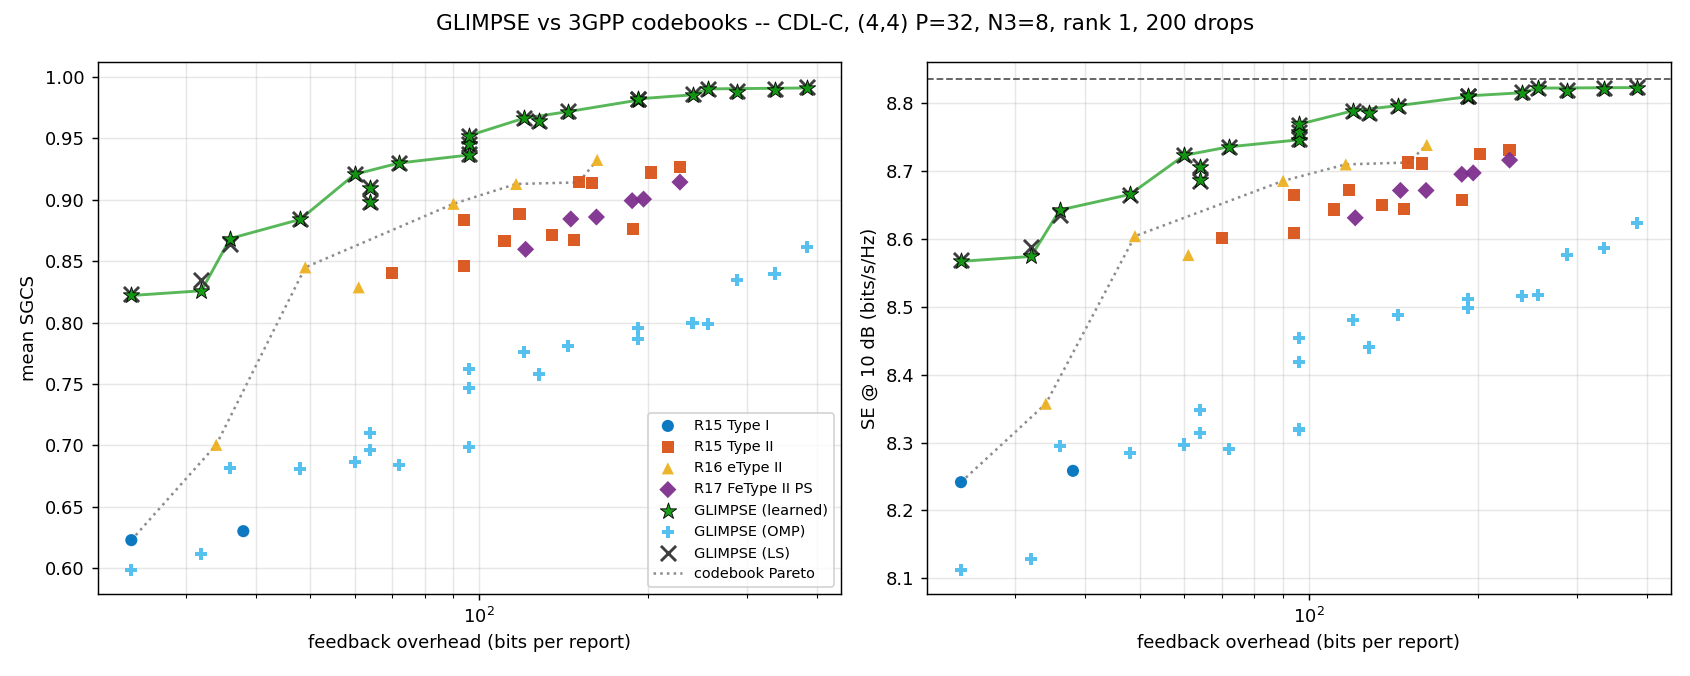
\includegraphics[width=0.98\textwidth]{figs/fig_glimpse_frontier.png}
\caption{Rate--distortion frontier, CDL-C, $(4,4)$ array, $P{=}32$, $N_3{=}8$, rank 1, 200 drops: mean SGCS (left) and SE at 10\,dB (right) vs.\ feedback bits, every codebook configuration plus GLIMPSE with the learned/OMP/LS decoders.}
\label{fig:frontier}
\end{figure*}

\subsection{Overhead at Matched Fidelity}
Table~\ref{tab:gain} and Fig.~\ref{fig:gain} give the feedback bits GLIMPSE and the cheapest codebook configuration each need to reach a target mean SGCS. GLIMPSE cuts overhead by \textbf{29--63\%}, with the largest reductions (48--63\%) at the high-fidelity operating points relevant to MU-MIMO pairing.

\begin{table}[t]
\centering
\caption{Feedback bits to reach a target mean SGCS, CDL-C}
\label{tab:gain}
\begin{tabular}{@{}lrrr@{}}
\toprule
Target SGCS & Codebook bits & GLIMPSE bits & Reduction \\
\midrule
0.70 & 34  & 24 & $-$29\% \\
0.80 & 49  & 24 & $-$51\% \\
0.85 & 90  & 36 & $-$60\% \\
0.90 & 116 & 60 & $-$48\% \\
0.92 & 162 & 60 & $-$63\% \\
\bottomrule
\end{tabular}
\end{table}

\begin{figure}[t]
\centering
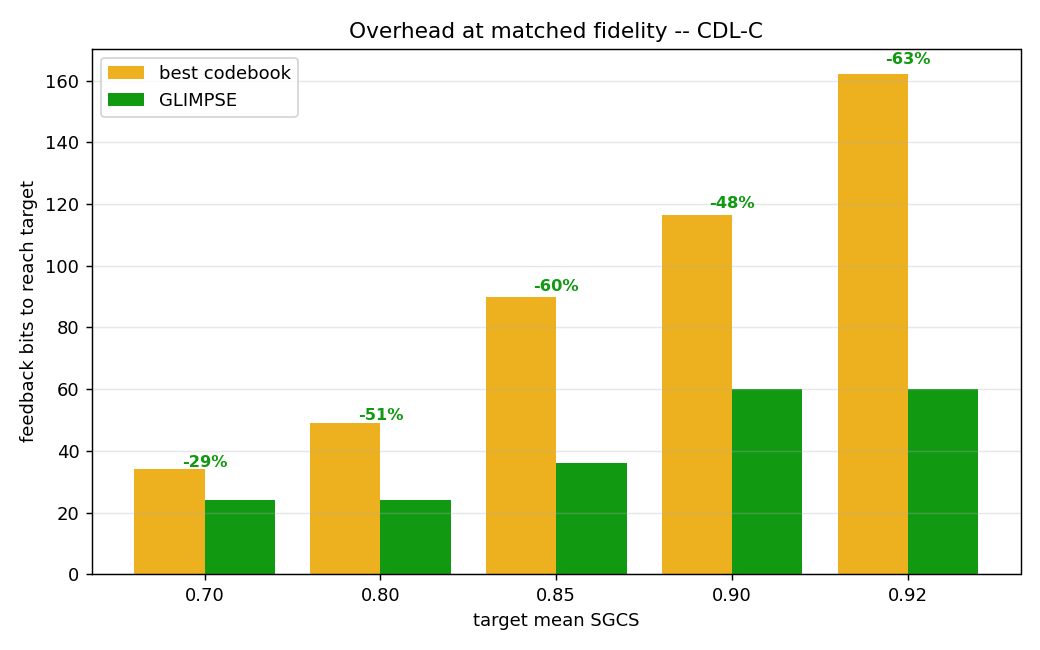
\includegraphics[width=0.98\linewidth]{figs/fig_glimpse_gain.png}
\caption{Overhead at matched fidelity, CDL-C: GLIMPSE vs.\ the best codebook configuration reaching the same target mean SGCS.}
\label{fig:gain}
\end{figure}

GLIMPSE also reaches mean SGCS \textbf{0.982 at 192 bits}, closing to within 0.025 bits/s/Hz of the eigen upper bound at 10\,dB SNR (within 0.013 by 256 bits) -- a fidelity no codebook configuration attains at any overhead in our sweep (best codebook $\approx$0.93). It further occupies the sub-40-bit regime the codebooks cannot enter: the smallest R16 report is 34 bits (SGCS 0.70), while GLIMPSE places continuous operating points down to 24 bits (SGCS 0.82, versus 0.62 for the 24-bit Type I report).

\subsection{Ablations: Where the Gain Comes From}
Figure~\ref{fig:ablation} isolates each design choice by changing one factor at a time. Replacing the fitted KLT basis with a distribution-blind random projection of the same size collapses mean SGCS from $\sim$0.95 to $\sim$0.07--0.10 at matched bits: at $m{=}16$ the KLT captures 93\% of the target energy against 6\% ($=m/D$) for the random basis, verified directly from the published basis matrix. \emph{This is the entire source of GLIMPSE's advantage over the codebooks} -- a measurement basis matched to the channel's second-order statistics rather than an assumed DFT grid. Reverse water-filling adds a smaller, consistent gain of $\approx$0.01--0.02 SGCS at matched bits over uniform bit allocation. Most notably, the linear least-squares decoder \eqref{eq:ls} matches the $\approx$0.22M-parameter learned decoder \eqref{eq:unroll} to three decimals across the entire in-distribution range (e.g.\ 0.9452 vs.\ 0.9450 at 96 bits): because the KLT is already the optimal linear sketch, little non-linear structure remains for the network to exploit in-distribution, and \textbf{GLIMPSE needs no neural network at the gNB at all}. Orthogonal matching pursuit, the classical compressed-sensing decoder, trails both by 0.15--0.30 SGCS -- its sparsity prior is a poor fit for the KLT's dense coordinates and it serves only as the guaranteed-convergence classical fallback.

\begin{figure}[t]
\centering
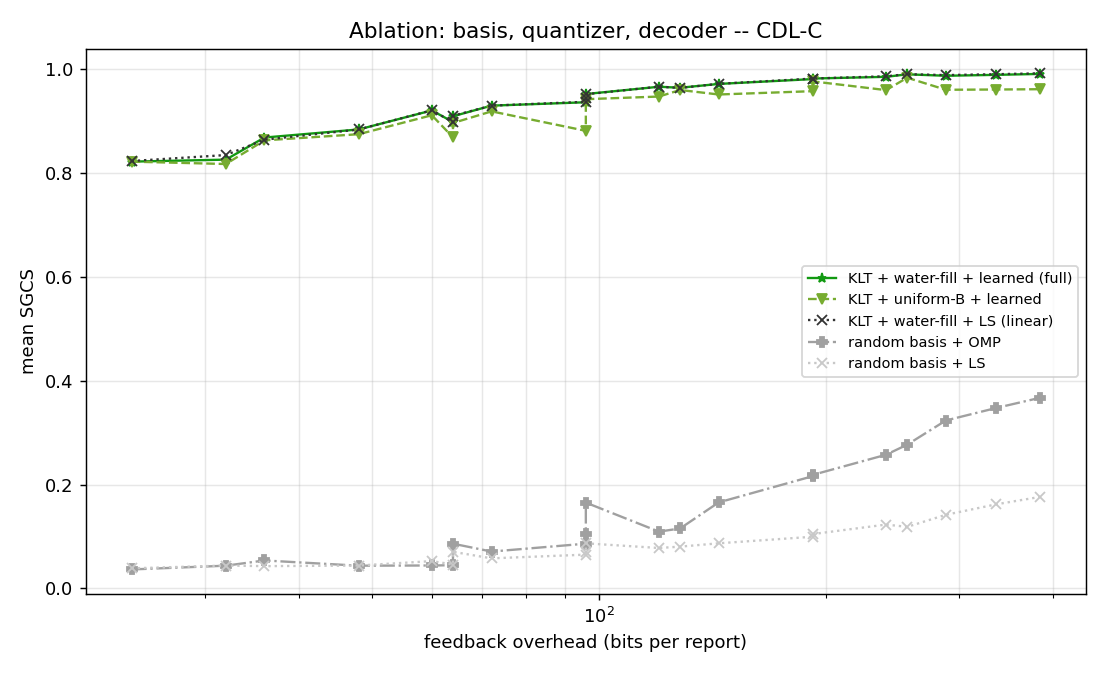
\includegraphics[width=0.98\linewidth]{figs/fig_glimpse_ablation.png}
\caption{Ablation on CDL-C: basis (KLT vs.\ random), quantizer (water-filled vs.\ uniform), and decoder (learned vs.\ LS vs.\ OMP), one factor changed at a time.}
\label{fig:ablation}
\end{figure}

\section{Cross-Profile Generalization, Limitations, and Positioning vs.\ Prior Art}
The KLT basis and decoder are fitted on the CDL-A/B/C mix. Figure~\ref{fig:models} evaluates GLIMPSE at a fixed $m{=}24$ ($\approx$144 bits) against the best codebook configuration within 15\% of that budget, across all five CDL profiles.

\begin{figure}[t]
\centering
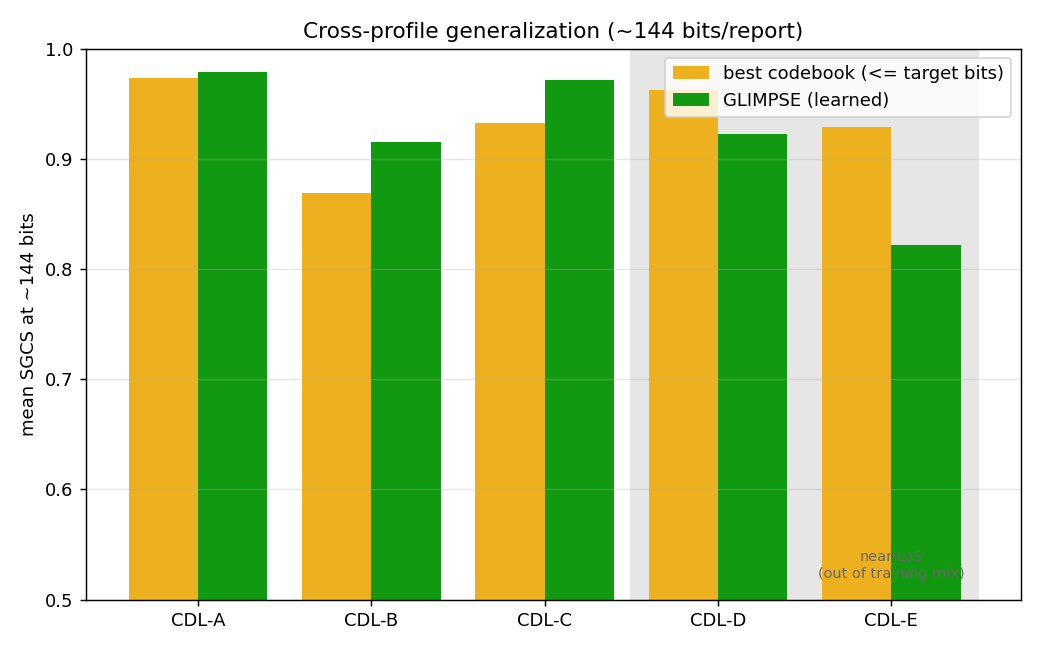
\includegraphics[width=0.98\linewidth]{figs/fig_glimpse_models.png}
\caption{Cross-profile generalization at $\approx$144 bits/report: GLIMPSE (learned) vs.\ the best nearby-budget codebook configuration, CDL-A through E. CDL-D/E are near-line-of-sight, outside the CDL-A/B/C training mix.}
\label{fig:models}
\end{figure}

On the three \textbf{in-distribution} profiles, GLIMPSE wins comfortably: 0.979 vs.\ 0.973 (CDL-A), 0.915 vs.\ 0.869 (CDL-B), 0.972 vs.\ 0.932 (CDL-C). On the two \textbf{out-of-distribution}, near-line-of-sight profiles -- dominated by a single specular path, statistically unlike the rich-scattering training mix -- the fixed-DFT codebooks \textbf{win}: 0.963 vs.\ 0.922 (CDL-D) and 0.929 vs.\ 0.822 (CDL-E). This is stated without varnish: it is the bias--variance cost of any statistically matched scheme. A codebook's basis assumes nothing about the channel distribution, so it neither gains from matching it nor loses from mismatching it; GLIMPSE's KLT is tuned to rich scattering and is the wrong basis for a near-line-of-sight channel.

This frames GLIMPSE's operating envelope honestly. It is a large win when the deployment distribution is known and reasonably stationary -- the common case for a fixed cell's scattering environment, and the implicit premise of any learned CSI scheme, including the two-sided autoencoder literature it improves upon. Where the distribution is unknown or includes a line-of-sight regime, two mitigations are available without any UE change: (i) train the KLT basis and decoder on a broader mix including LoS profiles, or (ii) fall back to the distribution-blind \texttt{basis="random"} variant, which forfeits peak efficiency for codebook-independent robustness (a Johnson--Lindenstrauss/rotation argument makes its measurements near-Gaussian for \emph{any} input distribution). A production system would detect the LoS regime -- which the UE already estimates for RI/CQI -- and fall back accordingly; GLIMPSE and the codebooks are complementary, not mutually exclusive. Two further caveats: the basis and decoder are fitted per antenna geometry $(N_1,N_2,N_3)$, a gNB-side standardization artifact rather than a UE burden but one that requires one basis/decoder per array configuration; and GLIMPSE reports the eigen-precoder exactly as Type II does, so it inherits the same CSI-aging behavior and does not itself predict future channel states.

\subsection{Positioning vs.\ Prior Art}
Table~\ref{tab:positioning} summarizes the comparison. Each ingredient in GLIMPSE exists in isolation -- KLT/PCA compression, transform-coding bit allocation~\cite{coverthomas2006,gershogray1992}, compressed-sensing feedback~\cite{kuo2012compressive,rao2014distributed}, unrolled reconstruction~\cite{gregorlecun2010} -- but composing them under the one-sided constraint, and benchmarking head-to-head against the \emph{full} R15--R17 codebook family on identical channels, is what yields simultaneously: a large fidelity/overhead gain in-distribution, the deployability of a codebook (a published constant matrix, no neural network required on either side), a continuous rateless overhead knob, and a well-characterized out-of-distribution failure mode with a principled fallback. Unlike CsiNet-family autoencoders~\cite{wen2018csinet,guo2020csinetplus,lu2020crnet,cui2022transnet}, nothing learned crosses the air interface or the vendor boundary.

\begin{table}[t]
\centering
\caption{Positioning vs.\ prior CSI feedback approaches}
\label{tab:positioning}
\small
\begin{tabular}{@{}p{1.5cm}p{1.6cm}p{0.7cm}p{2.9cm}@{}}
\toprule
Approach & UE cost & 2-sided? & Report format \\
\midrule
Type II codebooks & heavy beam/tap search & no & fixed grid, discrete ladder \\
CsiNet family~\cite{wen2018csinet,guo2020csinetplus,lu2020crnet,cui2022transnet} & full learned CNN/attention encoder & yes & learned latent \\
Classical CS~\cite{kuo2012compressive,rao2014distributed} & linear projection & no & random sketch \\
\textbf{GLIMPSE} & one $m\!\times\!D$ matmul & no & rateless KLT sketch \\
\bottomrule
\end{tabular}
\end{table}

\section{Conclusion}
GLIMPSE shows that the two deployment blockers of learned CSI feedback -- UE complexity and inter-vendor coordination -- are not intrinsic to learning-based gains but artifacts of putting the learned component on the wrong side of the air interface. By fitting the KLT basis of the channel eigenvector distribution offline and publishing it as a constant, GLIMPSE achieves a 29--63\% overhead reduction and a fidelity ceiling the 3GPP Type II family cannot reach, using an encoder cheaper than the codebook search it replaces and, in the headline configuration, no neural network anywhere in the pipeline. The honest limitation -- degraded performance under out-of-distribution near-LoS channels -- is a bias--variance trade-off common to any statistically matched scheme, and is mitigated by broader training or a distribution-blind fallback rather than by abandoning the approach. We see GLIMPSE as a template for one-sided learned CSI more broadly: keep the UE a fixed, published, spec-freezable pipeline, and put everything adaptive at the infrastructure, where it can be deployed, upgraded, and A/B-tested without a standardization body in the loop.

\bibliographystyle{IEEEtran}
\begin{thebibliography}{14}

\bibitem{3gpp38214}
3GPP, ``NR; Physical layer procedures for data,'' 3GPP TS 38.214, V19.4.0, Release 19.

\bibitem{kuo2012compressive}
P.-H. Kuo, H. T. Kung, and P.-A. Ting, ``Compressive sensing based channel feedback protocols for spatially-correlated massive antenna arrays,'' in \emph{Proc. 2012 IEEE Wireless Commun. Netw. Conf. (WCNC)}, Paris, France, 2012, pp. 492--497.

\bibitem{rao2014distributed}
X. Rao and V. K. N. Lau, ``Distributed compressive CSIT estimation and feedback for FDD multi-user massive MIMO systems,'' \emph{IEEE Trans. Signal Process.}, vol.~62, no.~12, pp. 3261--3271, 2014.

\bibitem{wen2018csinet}
C.-K. Wen, W.-T. Shih, and S. Jin, ``Deep learning for massive MIMO CSI feedback,'' \emph{IEEE Wireless Commun. Lett.}, vol.~7, no.~5, pp. 748--751, 2018.

\bibitem{guo2020csinetplus}
J. Guo, C.-K. Wen, S. Jin, and G. Y. Li, ``Convolutional neural network-based multiple-rate compressive sensing for massive MIMO CSI feedback: Design, simulation, and analysis,'' \emph{IEEE Trans. Wireless Commun.}, vol.~19, no.~4, pp. 2827--2840, 2020.

\bibitem{lu2020crnet}
Z. Lu, J. Wang, and J. Song, ``Multi-resolution CSI feedback with deep learning in massive MIMO system,'' in \emph{Proc. 2020 IEEE Int. Conf. Commun. (ICC)}, Dublin, Ireland, Jun. 2020, pp. 1--6.

\bibitem{cui2022transnet}
Y. Cui, A. Guo, and C. Song, ``TransNet: Full attention network for CSI feedback in FDD massive MIMO system,'' \emph{IEEE Wireless Commun. Lett.}, vol.~11, no.~5, pp. 903--907, 2022.

\bibitem{guo2022overview}
J. Guo, C.-K. Wen, S. Jin, and G. Y. Li, ``Overview of deep learning-based CSI feedback in massive MIMO systems,'' \emph{IEEE Trans. Commun.}, vol.~70, no.~12, pp. 8017--8045, 2022.

\bibitem{eckartyoung1936}
C. Eckart and G. Young, ``The approximation of one matrix by another of lower rank,'' \emph{Psychometrika}, vol.~1, no.~3, pp. 211--218, 1936.

\bibitem{lloyd1982}
S. P. Lloyd, ``Least squares quantization in PCM,'' \emph{IEEE Trans. Inf. Theory}, vol.~IT-28, no.~2, pp. 129--137, Mar. 1982.

\bibitem{max1960}
J. Max, ``Quantizing for minimum distortion,'' \emph{IRE Trans. Inf. Theory}, vol.~6, no.~1, pp. 7--12, Mar. 1960.

\bibitem{coverthomas2006}
T. M. Cover and J. A. Thomas, \emph{Elements of Information Theory}, 2nd ed. Hoboken, NJ, USA: Wiley-Interscience, 2006.

\bibitem{gershogray1992}
A. Gersho and R. M. Gray, \emph{Vector Quantization and Signal Compression}. Boston, MA, USA: Kluwer Academic Publishers, 1992.

\bibitem{gregorlecun2010}
K. Gregor and Y. LeCun, ``Learning fast approximations of sparse coding,'' in \emph{Proc. 27th Int. Conf. Mach. Learn. (ICML)}, Haifa, Israel, 2010, pp. 399--406.

\end{thebibliography}

\end{document}
